\documentclass[12pt]{article}
\usepackage[margin=1.1in]{geometry}
\usepackage{amsmath,amssymb,amsthm}
\usepackage[round]{natbib}
\usepackage{setspace}
% JCGS submission build: flip to \jcgstrue for double spacing
\newif\ifjcgs
\jcgsfalse
\ifjcgs\doublespacing\fi
\usepackage{graphicx}
\usepackage{booktabs}
\usepackage{algorithm}
\usepackage{algpseudocode}
\usepackage[hidelinks]{hyperref}
\hypersetup{pdftitle={Scalable Probit Share Calibration},
pdfauthor={Peter Cotton}}

\newtheorem{proposition}{Proposition}
\newtheorem{theorem}{Theorem}
\theoremstyle{remark}
\newtheorem{remark}{Remark}

\newcommand{\E}{\mathbb{E}}
\newcommand{\Prob}{\mathbb{P}}

\title{Scalable Probit Share Calibration}
\author{Peter Cotton\thanks{peter.cotton@microprediction.com. Every
number in this paper is produced by a committed, seeded script; see
Reproducibility and Supplementary Materials.}}
\date{August 2026}

\begin{document}
\maketitle

\begin{abstract}
Probit models are a cornerstone of economic, choice, and contest theory, and
machine learning runs on the same latent-utility family. Yet the
many-alternative form sees little use beyond small menus: its probabilities
have no closed form, standard smooth orthant evaluators price one
alternative at a time, and calibration, meaning the recovery of the utilities at which model
shares match observed shares with the factor covariance given and fixed,
has been out of reach at scale. We give an
algorithm that calibrates a two-factor probit model with a thousand
alternatives in three seconds on a laptop, with wall time approximately
linear in the number of alternatives over the tested range. Relative to
a plain direct-Monte-Carlo simulation-in-the-loop benchmark, measured
throughput and standard sampling-error arithmetic imply a speed
advantage of roughly six orders of magnitude at matched share-map
accuracy. The computed shares carry log-share errors of a few parts in
a hundred thousand, hundred-to-one shares included.
\end{abstract}

\noindent\textbf{Keywords:} multinomial probit; discrete choice;
numerical quadrature; Jacobian--vector product; share inversion; factor
model

\section{Introduction}

Probit models are a cornerstone of economic, choice, and contest theory:
Thurstone's comparative judgment, the ordered and binary probits of applied
microeconometrics, and the Lazear--Rosen tournament
\citep{lazear1981} are all the same
Gaussian latent-performance model. Machine learning runs on the same
family: a softmax output layer is its Luce--Gumbel member, and
Thurstone--Mosteller pairwise comparison \citep{mosteller1951}, the
probit member, underlies
rating systems and preference learning.

Such models are calibrated to observed shares so that the recovered
utilities can answer questions the data do not: elasticities, welfare,
pricing, the effect of adding or removing an alternative. The models used
for this, essentially universally, are the logit family: multinomial logit,
nested logit, and above all random-coefficients logit in the BLP tradition
\citep{berry1995,train2009,conlon2020}. They are universal for one reason.
They can be computed.

Choice modeling did not start there: it started with Thurstone's 1927 model
\citep{thurstone1927} of jointly Gaussian utilities with unrestricted
correlation, brought into econometrics as the conditional (multinomial)
probit model by \citet{hausman1978} and known since as MNP. The same
object has re-emerged in machine learning: conditional on an input,
heteroscedastic image classifiers place exactly this
low-rank-plus-diagonal Gaussian race on their final layer and take the
argmax, approximating the winner probabilities by Monte Carlo over a
softmax relaxation \citep{collier2021}.

Probit probabilities are $(N-1)$-dimensional Gaussian integrals with no
closed form. The standard evaluator is the Geweke--Hajivassiliou--Keane
(GHK) simulator \citep{geweke1994,hajivassiliou1998,train2009}, the
econometric branch of the Genz separation-of-variables family
\citep{genz1992} whose RQMC form (Genz--Bretz) is the default in
computational statistics: it writes
the probability that alternative $i$ beats the rest as an orthant
probability of the difference utilities, and estimates it by sampling
truncated normals sequentially along a Cholesky factor. That is a separate simulation per alternative, with $R^{-1/2}$ error in
the number of draws, and it is why probit survives mainly on small menus:
the field kept the computable models and gave up the model it started
from.

The concession is not free. Logit-family substitution is structurally
restricted, and the calibration apparatus that demand estimation is built
on is routine only on the logit side. One measure of the cost, from one deliberately misspecified synthetic
design with oracle factor loadings (Section~\ref{sec:boundary}): in the
largest-deletion stratum, across twenty designs with every marginal
variance held at one, plain logit misallocates a median 25\% of the
demand released by a deleted alternative, against 1\% for factor probit
(experiment 29), the
closest of the four candidate structures.

This paper's point is that the barrier is not real for an important
class of covariance structures, the low-rank-plus-diagonal factor model
$\Sigma = VV^\top + \mathrm{diag}(D)$. The goal is \textbf{calibration}: given
observed shares and a fixed, known factor structure $(V, D)$, recover the
utilities at which the probit model reproduces them.

This is the probit
analogue of the inversions demand estimation runs on the logit side every
day \citep{berry1995,conlon2020}; estimating $(V, D)$ is the outer problem,
discussed in Section~\ref{sec:discussion}.

We solve it at $N = 1000$
in three seconds. The tractability objection that made the logit family
universal does not apply to factor-structured probit. The inverse
problem is also globally well-posed
(Proposition~\ref{thm:inv}: shares determine utilities uniquely up to
location). Three ingredients make it work:

\begin{enumerate}
\item \textbf{A fast forward map} (utilities $\to$ shares): all $N$
probabilities at once in $O(QNL)$ for $Q$ factor nodes and $L$ lattice
points. Calibration needs many forward evaluations; this is what makes
them affordable.
\item \textbf{Resampling-free derivatives}: Jacobian--vector products in
$O(QNL)$; in max-wins coordinates the Jacobian is a weighted graph
Laplacian, so reduced systems are symmetric positive definite. This supports
implicit differentiation and Newton--Krylov solvers; the calibration
reported below uses a cheaper damped Jacobi iteration.
\item \textbf{A single shared construction}: conditionally on the $k$
factors the alternatives are independent, and a lattice survival-product
identity computes every alternative's integral from one \emph{shared
survival field}, built once and reused for shares, slopes, and all $N$
single-removal counterfactuals.
\end{enumerate}

\paragraph{Prior art.} The nearest methods, and what each lacks:

\begin{center}
\footnotesize
\setlength{\tabcolsep}{4pt}
\begin{tabular}{p{4.4cm} p{4.4cm} p{4.6cm}}
\toprule
approach & all $N$ shares & calibration \\
\midrule
GHK simulation \citep{geweke1994,hajivassiliou1998} & $N$ separate runs, $R^{-1/2}$ (plain MC) & no reported large-$N$ share inversion known to us \\
direct utility simulation & whole vector per draw, $R^{-1/2}$ & raw frequency map is nonsmooth \\
analytic approximations \citep{bhat2011,connors2014} & per-alternative & no \\
factor quadrature \citep{butler1982,elrod1995} & $N$ separate $(k{+}1)$-dim integrals & no \\
Bayesian factor MNP \citep{loaiza2022} & simulation inside estimation & posterior, not a share map \\
neural amortization \citep{huch2026} & learned approximation, no prescribed tolerance & no \\
BLP-side inversion \citep{berry1995,conlon2020} & --- & logit family only \\
\textbf{this paper} & one $O(QNL)$ pass & Prop.~\ref{thm:inv}; 3\,s at $N{=}1000$ \\
\bottomrule
\end{tabular}
\end{center}

Figure~\ref{fig:scaling} shows calibration wall time as the number of
alternatives grows: roughly linear, three seconds at a thousand
alternatives and forty at ten thousand in the compiled implementation.

\begin{figure}[t]
\centering
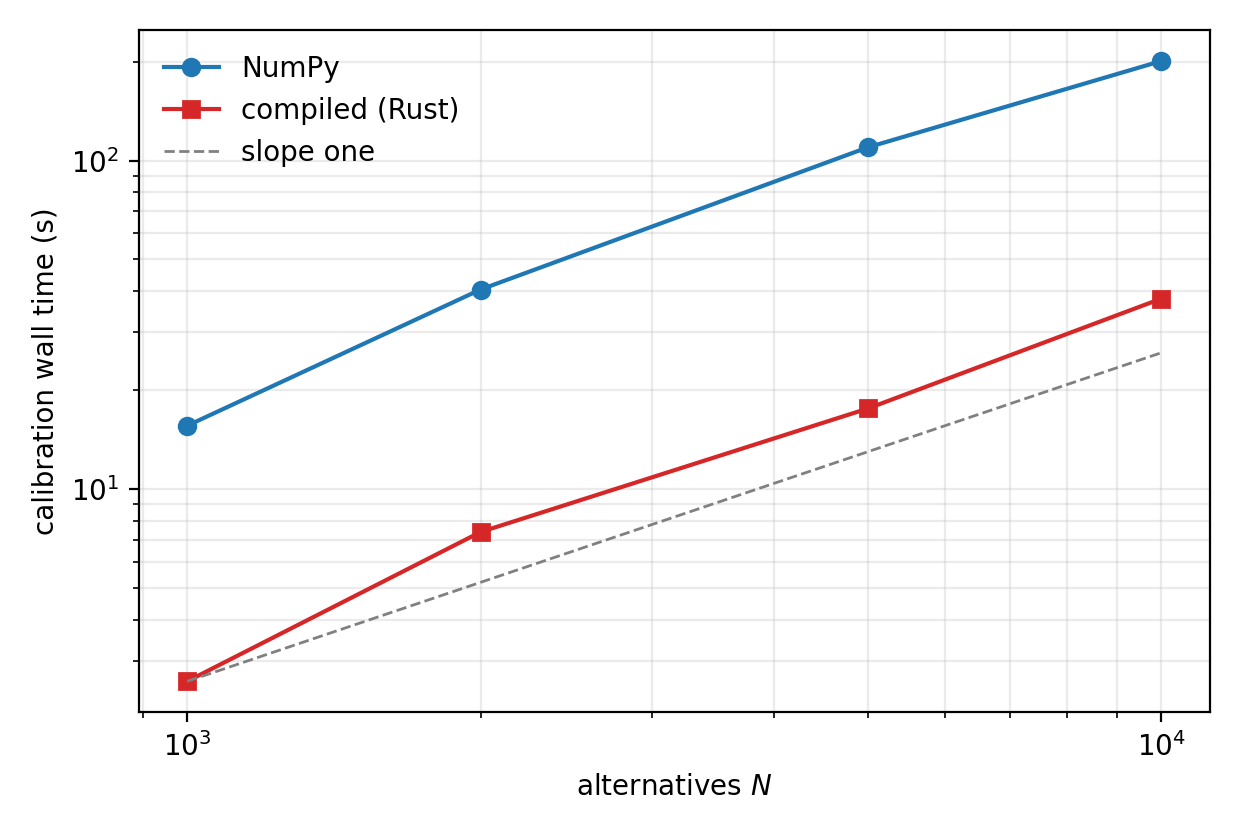
\includegraphics[width=0.62\textwidth]{figs/calibration_scaling.png}
\caption{Wall time to calibrate the full utility vector from target
shares ($k=2$ factors, independent $5\times10^6$-draw targets, experiment
19). Both implementations grow roughly linearly in $N$; the dashed guide
has slope one.}
\label{fig:scaling}
\end{figure}

\paragraph{Scope.} The method needs the factor form: where $\Sigma$ has no
adequate low-rank-plus-diagonal approximation in the choice-relevant quotient
space, simulation at exact $\Sigma$ remains the tool
(Section~\ref{sec:boundary}). The decisive advantages are precision,
reproducibility, resampling-free derivatives, and the calibration
machinery.

The one-pass identity comes from an unlikely literature: inferring ability
from win probabilities in multi-entrant races \citep{cotton2021}. That is
perhaps why it has not been assembled for probit before, despite each
ingredient being classical.

The factor structure is not a convenience grafted onto probit: it is
the original econometric model. \citet{hausman1978} induced correlation
through random taste coefficients, giving a covariance that is exactly
low-rank plus diagonal with observed attributes as loadings; freeing the
loadings is the factor-analytic MNP that \citet{mcfadden1984} proposed
precisely to reduce the dimension of the integral.

\paragraph{Model.} Throughout,
\begin{equation}
U_i \;=\; \mu_i + v_i^\top f + \sqrt{D_i}\,\varepsilon_i,
\qquad f \sim N(0, I_k), \quad \varepsilon_i \sim N(0,1) \text{ i.i.d.},
\quad D_i > 0,
\label{eq:model}
\end{equation}
i.e.\ $\Sigma = VV^\top + \mathrm{diag}(D)$; the chosen alternative is the
argmax of $U$. Throughout, $(V, D)$ is supplied and held fixed;
calibration solves for $\mu$ alone.

Factor dimension reduction for probit
is classical:
one-factor quadrature goes back to \citet{butler1982},
and factor-analytic probit to \citet{elrod1995}. The
contribution is the all-alternatives assembly, the inverse transform, the
derivative structure, and evidence for all of it.

\begin{proposition}[Conditional identity]\label{prop:identity}
Under \eqref{eq:model}, with $g_i(\cdot \mid f)$ and $F_i(\cdot \mid f)$
the conditional density and CDF of $U_i$ given $f$,
\begin{equation}
p_i \;=\; \E_f\!\left[\;\int g_i(x \mid f)
\prod_{j \neq i} F_j(x \mid f)\, dx \right],
\qquad \sum_i p_i = 1,
\label{eq:forward}
\end{equation}
and the product over $j \ne i$, for all $i$ simultaneously, is obtained from
$\log F_{\mathrm{field}} = \sum_j \log F_j$ by subtraction.
\end{proposition}
\begin{proof}
Conditional on $f$ the $U_j$ are independent, so $\Prob(U_i \text{ maximal}
\mid f) = \int g_i \prod_{j\ne i} F_j\,dx$; average over $f$. The events
partition (ties are null for continuous laws), giving $\sum_i p_i = 1$.
\end{proof}

\begin{proposition}[Complexity]\label{prop:complexity}
With $Q$ factor nodes and $L$ lattice points, the forward share vector
costs $O(QN(k+L))$, which is $O(QNL)$ for $k \ll L$; the full
single-removal ensemble $\{P(j \text{ chosen} \mid i
\text{ removed})\}_{i,j}$ costs $O(QN^2L)$ arithmetic and $O(N^2)$ storage,
reusing one conditional field construction.
\end{proposition}
\begin{proof}
Per node: the conditional locations cost $O(Nk)$, the field log-product
$O(NL)$, and each alternative's integral $O(L)$ after subtraction, giving
$O(N(k+L))$; the removal ensemble evaluates $N$
survivor integrals for each of $N$ removals, $O(N^2L)$, over the same cached
field.
\end{proof}

\begin{proposition}[Identification and differentiability]\label{prop:ident}
$p(\mu + c\mathbf{1}) = p(\mu)$, so $J = \partial p/\partial \mu$ has
$\mathbf{1}$ in its null space and $\mu$ is identified only up to location.
With $B$ an $N \times (N-1)$ basis of $\mathbf{1}^\perp$ and $\mu = B\eta$,
share inversion and implicit differentiation are taken in reduced coordinates:
$d\eta/d\theta = -(B^\top J B)^{-1} B^\top \partial p/\partial\theta$,
provided $B^\top J B$ is nonsingular.
\end{proposition}
\begin{proof}
For the invariance, write $U_i = \mu_i + \xi_i$ with $\xi_i = v_i^\top f
+ \sqrt{D_i}\,\varepsilon_i$. For every realization of the shocks,
$\arg\max_i (\mu_i + c + \xi_i) = \arg\max_i (\mu_i + \xi_i)$, since
adding $c$ to every coordinate changes no pairwise comparison. The choice
events therefore coincide realization by realization, so $p(\mu +
c\mathbf{1}) = p(\mu)$ for all $c$. Differentiating this identity in $c$
at $c = 0$ gives $J\mathbf{1} = 0$: the ones vector lies in the null space
of $J$, and two utility vectors differing by a common shift produce
identical shares, so $\mu$ is identified at most up to location.

For the reduced formula, suppose $\eta(\theta)$ satisfies the calibration
identity $p(B\eta(\theta), \theta) = \hat p$ on an open set of
$\theta$. Total differentiation gives the $N$-equation system
\[
J B \,\frac{d\eta}{d\theta} + \frac{\partial p}{\partial \theta}
= 0 .
\]
Only $N - 1$ of these equations are independent, but none are lost by
projecting: shares sum to one identically in both arguments, so
differentiating $\mathbf{1}^\top p = 1$ gives $\mathbf{1}^\top J = 0$
and $\mathbf{1}^\top (\partial p / \partial \theta) = 0$; both terms
already lie in $\mathbf{1}^\perp$, so the system is equivalent to its
image under $B^\top$. That image is $(B^\top J B)\, d\eta/d\theta =
-B^\top \partial p/\partial\theta$, and when $B^\top J B$ is
nonsingular (established for this model in Proposition~\ref{thm:inv}) it
inverts to the displayed formula, with local existence and smoothness of
$\theta \mapsto \eta(\theta)$ supplied by the implicit function theorem.
\end{proof}
\begin{proposition}[Shares determine utilities]\label{thm:inv}
For model \eqref{eq:model} with $D_i > 0$ and fixed known $(V, D)$, in
max-wins coordinates, define
for $i \ne j$
\[
w_{ij} \;=\; \E_f \int g_i(x \mid f)\, g_j(x \mid f)
\prod_{\ell \ne i,j} F_\ell(x \mid f)\, dx \;>\; 0 .
\]
Then $J = \partial p / \partial \mu$ satisfies $J_{ij} = -w_{ij}$ and
$J_{ii} = \sum_{j \ne i} w_{ij}$, i.e.
\[
J \;=\; \sum_{i<j} w_{ij} (e_i - e_j)(e_i - e_j)^\top,
\qquad
h^\top J h \;=\; \sum_{i<j} w_{ij} (h_i - h_j)^2 ,
\]
a weighted graph Laplacian with everywhere-positive weights: $J$ is symmetric,
positive semidefinite, has $\mathbf{1}$ as its only null direction, and
$B^\top J B \succ 0$ for every full-rank basis $B$ of $\mathbf{1}^\perp$.
Moreover $p = \nabla G$ for the social-surplus function
$G(\mu) = \E \max_i \{\mu_i + \xi_i\}$ (the Williams--Daly--Zachary /
McFadden identity \citep{williams1977,daly1978,mcfadden1981}), and the restriction of $p$ to
$\mathbf{1}^\perp$ is a smooth bijection onto the interior of the
probability simplex: every strictly positive target $\hat p$ has exactly one
mean-zero utility vector.
\end{proposition}
\begin{proof}
Start from \eqref{eq:forward}. For $j \ne i$, the parameter $\mu_j$
enters $p_i$ only through the factor $F_j(x \mid f) = \Phi\big((x - \mu_j
- v_j^\top f)/\sqrt{D_j}\big)$, whose $\mu_j$-derivative is $-g_j(x \mid
f)$. Differentiating under the integral is justified by a uniform bound:
$\int g_i(x \mid f)\, g_j(x \mid f)\, dx = \exp[-(m_i(f) -
m_j(f))^2 / (2(D_i + D_j))] / \sqrt{2\pi(D_i + D_j)} \le 1 /
\sqrt{2\pi(D_i + D_j)}$, uniform in $f$ and $\mu$, so dominated
convergence applies and gives
\[
J_{ij} \;=\; \frac{\partial p_i}{\partial \mu_j}
\;=\; -\,\E_f \int g_i(x \mid f)\, g_j(x \mid f)
\prod_{\ell \ne i,j} F_\ell(x \mid f)\, dx \;=\; -\,w_{ij},
\]
and the integrand is symmetric in $(i, j)$, so $J_{ij} = J_{ji}$. For the
diagonal, translation invariance ($p(\mu + c\mathbf{1}) = p(\mu)$,
Proposition~\ref{prop:ident}) gives $J\mathbf{1} = 0$, hence $J_{ii} =
-\sum_{j \ne i} J_{ij} = \sum_{j \ne i} w_{ij}$; the adding-up
identity $\mathbf{1}^\top J = 0$ follows separately from
$\mathbf{1}^\top p = 1$, or from symmetry. (The same diagonal follows directly: $\partial_{\mu_i} g_i =
-g_i'$, and integrating by parts, $\int (-g_i') \prod_{j \ne i} F_j\,dx
= \int g_i \sum_{j \ne i} g_j \prod_{\ell \ne i,j} F_\ell\,dx$, the
boundary terms vanishing because $g_i \to 0$ at $\pm\infty$ while the
product stays bounded.) Positivity of the weights: for every $f$ and $x$
the Gaussian densities $g_i, g_j$ are strictly positive, and each
$F_\ell(x \mid f)$ is strictly positive for finite $x$, so the integrand
is strictly positive on all of $\mathbb{R}$ and $w_{ij} > 0$.

With $J_{ij} = -w_{ij}$ off the diagonal and $J_{ii} = \sum_{j \ne i}
w_{ij}$, expanding $\sum_{i<j} w_{ij}(e_i - e_j)(e_i - e_j)^\top$ entry by
entry reproduces $J$, and therefore $h^\top J h = \sum_{i<j}
w_{ij}(h_i - h_j)^2 \ge 0$. Because every $w_{ij}$ is strictly positive,
the form vanishes only when $h_i = h_j$ for all pairs, i.e.\ for constant
$h$: $J$ is positive semidefinite with null space exactly
$\mathrm{span}\{\mathbf{1}\}$, hence positive definite on
$\mathbf{1}^\perp$. For inversion, minimize $H(\mu) = G(\mu) - \hat p^\top
\mu$ over $\mathbf{1}^\perp$: $H$ is strictly convex there (its Hessian is
the reduced $J$), and since the shocks have zero mean, $G(\mu) \ge \max_i
\mu_i$, so
\[
H(\mu) \;\ge\; \max_i \mu_i - \hat p^\top \mu
\;=\; \textstyle\sum_i \hat p_i (\max_j \mu_j - \mu_i)
\;\ge\; \hat p_{\min} \,(\max_i \mu_i - \min_i \mu_i)
\;\ge\; \hat p_{\min}\, \|\mu\|_2 / \sqrt{N}
\]
on $\mathbf{1}^\perp$, where the last step uses that a zero-sum vector has
$\max_i \mu_i \ge 0 \ge \min_i \mu_i$, so the range dominates
$\|\mu\|_\infty \ge \|\mu\|_2/\sqrt{N}$; hence $H$ is coercive. Since $D_i > 0$ the
utilities have a smooth full-support joint density and ties are null, so
differentiating under the expectation gives $\nabla G = p$. At the unique
constrained minimizer, $B^\top(p(\mu) - \hat p) = 0$, so $p(\mu) - \hat
p \in \mathrm{span}\{\mathbf{1}\}$; both vectors sum to one, so the
coefficient is zero and $p(\mu) = \hat p$. Smoothness of the inverse
follows from the inverse-function theorem, since $B^\top J B \succ 0$
everywhere.
\end{proof}
\begin{remark}[The photo-finish graph]
In English: $w_{ij}$ is the probability density of a photo-finish between
$i$ and $j$, a tie for the win with everyone else behind, and moving
utility from $j$ to $i$ moves share along every photo-finish edge at
exactly that rate. The alternatives form a \emph{photo-finish graph}:
complete, with strictly positive weights, because Gaussian utilities give
every pair a strictly positive tie density at the winning frontier. The proposition's conclusions are then
graph facts. Constants span the null space because the quadratic form
$\sum_{i<j} w_{ij}(h_i - h_j)^2$ sees only differences: shares cannot
identify the overall utility level, only gaps, which is economically
obvious and here algebraically automatic.

Positive weights make the graph
connected, so the constant vector is the \emph{only} null direction, the
gradient map is strictly monotone as an operator on $\mathbf{1}^\perp$
(not coordinatewise), and shares determine utilities uniquely.

And symmetry plus positive definiteness make every
reduced Newton system SPD, so conjugate gradients apply with the $O(QNL)$
Jacobian--vector product of Proposition~\ref{prop:jvp} playing the role of
a fast Laplacian multiply. Structurally, each linearization of the calibration solves a weighted
graph-Laplacian system on the photo-finish graph (the weights themselves
move with $\mu$), and such systems admit mature SPD and
graph-Laplacian solvers for the same reason resistor
networks and heat equations are.

None of this is specifically Gaussian.
Any conditionally independent additive random-utility race with
everywhere-positive smooth densities has, under the corresponding
integrability and differentiability conditions (finite social surplus,
differentiation under the integral), a weighted-Laplacian Jacobian and an
interior-simplex diffeomorphism modulo translation. Gaussian factor
probit is the computationally important specialization.
\end{remark}
\begin{remark}
Social-surplus convex duality for discrete choice is classical
\citep{chiong2016,norets2013}; what is new here is not well-posedness but its
scalable realization. The conjugate view makes that precise. $G$ is
convex with $p = \nabla G$, so $\Omega = G^*$ is a convex regularizer on
the simplex and $p(\mu) = \arg\max_{q \in \Delta}\{\mu^\top q -
\Omega(q)\}$. For iid Gumbel noise $\Omega$ is Shannon negentropy and
the maximizer is softmax; in general it is the generalized entropy of
\citet{fosgerau2020}, with the perturbation--regularization duality
developed for machine learning by \citet{berthet2020}. Factor probit
carries a covariance-dependent, nonseparable entropy that couples
alternatives through the factor structure, and this paper's three
algorithms are the three faces of that dual pair: the transform
evaluates $\nabla G$, calibration evaluates the mirror map $\mu =
\nabla\Omega(p)$ on the mean-zero quotient, and the Jacobian--vector
product applies the Hessian $\nabla^2 G$. Each is built from the same
$O(QN(k+L))$ primitive: the forward map is one pass, each
Jacobian--vector product is one pass, and each calibration iteration is
one pass (total calibration cost multiplies by the iteration count,
typically 10--15). On the simplex, $\nabla\Omega(p)$ is an equivalence
class modulo constants; its mean-zero representative is the calibrated
utility. The bijection itself is essentially known:
injectivity up to a common shift is the Hotz--Miller inversion
\citep{hotz1993}, surjectivity is \citet{norets2013}, and
\citet{bgh2013} derive demand invertibility from
connectivity of the substitution structure, the same mechanism as the
photo-finish graph; the compact proof above keeps the Gaussian factor
case self-contained and exhibits the weights the algorithm uses. Each
identity in the proposition is also checked
numerically in the repository: the $w_{ij}$ representation against finite
differences to $6\times10^{-9}$, symmetry to $4\times10^{-12}$, and
positive definiteness of the reduced numerical Jacobian.
\end{remark}

\begin{remark}[Transport form]
On the contrast space, with $b_i = e_i - \mathbf{1}/N$ the vertices of
a regular simplex, $\arg\max_i (x_i + \mu_i) = \arg\min_i
\{\tfrac12 \|x - b_i\|^2 - \mu_i\}$: the choice cells are the
Laguerre cells of quadratic semi-discrete optimal transport from the
contrast Gaussian to $\nu_q = \sum_i q_i \delta_{b_i}$, and
Kantorovich duality identifies $\Omega(q)$, up to an additive constant,
with $\tfrac12 W_2^2$ between them. Calibration is the dual solve of a
structured transport problem; $w_{ij}$ is the Gaussian surface mass on
the shared Laguerre facet (scaled by $1/\sqrt2$), and a Newton step is
an electrical solve on that network, for which
Proposition~\ref{prop:jvp} is the matrix-free multiply.

Gaussian integration by parts closes the conjugate in graph form:
$G(\mu) = \mu^\top p + \mathrm{tr}(\Sigma J)$, hence
\[
\Omega(p) = -\mathrm{tr}(\Sigma J)
= -\sum_{i<j} w_{ij}\, s_{ij}^2, \qquad
s_{ij}^2 = D_i + D_j + \|v_i - v_j\|^2 :
\]
the generalized entropy is the negative variance-weighted total
conductance of the photo-finish graph (binary check
$\Omega = -s\,\phi(\Phi^{-1}(q))$ to $3\times10^{-13}$; the identity to
$3\times10^{-9}$; experiment 27). Common covariance shifts vanish on
every edge difference, which is the quotient statement once more. The
assignment form of $G^*$ is classical \citep{chiong2016}; the
regular-simplex quadratic specialization and its $O(QN(k+L))$
value--gradient--Hessian oracle are developed in a companion note.
\end{remark}

\begin{proposition}[Jacobian--vector products in $O(QNL)$]\label{prop:jvp}
With hazards $\lambda_j = g_j / F_j$, $\Lambda = \sum_j \lambda_j$, and
$A = \sum_j h_j \lambda_j$ (all conditional on $f$, all functions of $x$),
the Jacobian of the exact max-wins map acts on a direction $h$ as
\[
(Jh)_i \;=\; \E_f \int g_i \Big(\prod_{j \ne i} F_j\Big)
\left( h_i \Lambda - A \right) dx ,
\]
where the field sums $\Lambda$ and $A$ are formed once per node and lattice
point, so all $N$ components cost $O(NL)$ per node. In English: a direction
$h$ perturbs alternative $i$'s share only through the gap between its own
hazard weight $h_i \Lambda$ and the field average $A$. Translation
invariance is visible ($h = \mathbf{1}$ gives $A = \Lambda$, hence $Jh =
0$), and the weighted-Laplacian form of Proposition~\ref{thm:inv} follows by
expanding $A$.
This enables Krylov solves of the reduced system in
Proposition~\ref{prop:ident} without forming $J$ densely at $O(QN^2L)$.
\end{proposition}
\begin{proof}
Write $R_i = \prod_{j \ne i} F_j$. For the own derivative,
$\partial_{\mu_i} g_i(x) = -g_i'(x)$ (a location shift), and integrating by
parts, $\int (-g_i') R_i\,dx = \int g_i R_i' \,dx = \int g_i R_i
\sum_{j \ne i} \lambda_j\,dx = \int g_i R_i (\Lambda -
\lambda_i)\,dx$. For $j \ne i$, $\partial_{\mu_j} F_j = -g_j$, so the
cross derivative is $-\int g_i g_j \prod_{\ell \ne i,j} F_\ell\,dx =
-\int g_i R_i \lambda_j\,dx$. Summing against $h$,
$(Jh)_i = \int g_i R_i [\,h_i(\Lambda - \lambda_i) - \sum_{j \ne i}
h_j \lambda_j\,]dx = \int g_i R_i (h_i \Lambda - A)\,dx$; average over
$f$.
\end{proof}

\paragraph{The differentiated map.} Three maps must be
distinguished: the exact max-wins map $p^{\max}(\mu)$; the reflected
min-wins map $p^{\min}(a)$ used by the implementation, related by $a = -\mu$
so that $D_\mu p^{\max}[h] = D_a p^{\min}[-h]$; and the implemented
approximation $p_{Q,L} = \tilde p_{Q,L} / (\mathbf{1}^\top \tilde
p_{Q,L})$, whose derivative carries a normalization correction: with $v =
D\tilde p[h]$ and $s = \mathbf{1}^\top \tilde p$,
\[
D p_{Q,L}[h] \;=\; \frac{v - p_{Q,L}\, (\mathbf{1}^\top v)}{s}.
\]
The correction vanishes for the continuum map and is numerically
negligible at the resolutions tested. A further distinction: integration by parts is a continuum identity, so the Laplacian
formula of Proposition~\ref{prop:jvp} is the exact derivative of the
\emph{continuum} map, not of the finite rectangle sum.

The exact derivative
of the frozen-grid sum replaces the own-term by $(x - m_i)/D_i$ (no
integration by parts), costs the same $O(QNL)$, and ships in the repository
(\texttt{form="grid"}).

Measured at $L = 1501$ (the derivative-comparison resolution) the
two forms agree to $1.7\times10^{-14}$; at $L = 51$ the continuum form is
off by $2.6\times10^{-5}$ while the grid form still matches finite
differences.

So the Laplacian form is an extremely accurate symmetric surrogate at the
resolutions used, and exact differentiation of the normalized
\emph{frozen-grid} map is available when needed; the returned adaptive map
additionally moves its envelope with $\mu$, a tail effect measured below
$10^{-8}$ at $L = 1501$.

The implemented inversion rebuilds the lattice envelope from the current
utilities at each iteration, holds it fixed within the iteration, and
projects the utilities to mean zero after every update
(Algorithm~\ref{alg:calibrate}).

\paragraph{Tail-stable implementation.} Tail stability requires the log
domain throughout: $\log \Phi$ evaluated directly (forming $1 - \Phi(z)$
by literal subtraction rounds to zero near $z \approx 8.3$ through
cancellation), the analytic $\log g$, and hazards as $\exp(\log g - \log
\Phi)$; the Gaussian inverse Mills ratio is unbounded but grows only
linearly in the extreme tail, rather than exponentially, which is the
numerically important property.

Flooring a density before taking its logarithm while the exact
log-survival stays finite produces spurious $e^{+92}$ hazards on problems as
mild as $N = 8$ with heterogeneous $D$; that configuration is a regression
test. In the forward map the same discipline lets deep-tail shares resolve to
genuine small positives rather than floored zeros.

\paragraph{Beyond Gaussian factors.} The factors need not be Gaussian: \eqref{eq:forward} requires only
conditional independence and an integrable factor law, so Student, mixture,
or empirical factor distributions are admissible with appropriate nodes, and
the base densities may be arbitrary and alternative-specific. One caution for
asymmetric laws: the implementation works in the reflected (min-wins)
race, and $-U$ has the same distribution as the reflected model only when the
factor and base laws are symmetric; for asymmetric laws the reflected
distributions must be used explicitly.

\paragraph{Numerical method.} Unless otherwise stated, forward and
calibration runs use $L = 501$ lattice points, chosen from the measured
lattice sweep (experiment 17 spans $L = 101$ to $6001$;
self-convergence reaches machine precision by $L \approx 200$). The
derivative comparison below uses $L = 1501$, and higher-resolution
reference calculations use $L = 3001$ or $5001$. The lattice sits on
the adaptive interval
$[\min_{i,q} m_i(f_q) - 8\max_i\sqrt{D_i},\,
\max_{i,q} m_i(f_q) + 8\max_i\sqrt{D_i}]$, where $q = 1, \dots, Q$ indexes
the retained factor nodes.

Factor integration: the main experiments use product
Gauss--Hermite of order 15/11/9 for $k = 2/3/4$; the boundary experiment
(experiment 14) uses order 15 per dimension for all $k \le 4$, which after
pruning weights below $10^{-7}$ of the maximum leaves $Q = 145$, $1317$, and
$10929$ nodes for $k = 2, 3, 4$, making the exponential growth of $Q$
with rank explicit. Scrambled-Sobol nodes ($2^{13}$ points, fixed seed) are used
for $k > 4$: fixed-node and reproducible (a fixed-seed randomized Sobol
construction), rather than deterministic in the strict sense.

Survival floors sit at $10^{-300}$ and the quadrature output is normalized by
its sum. The returned map is a reproducible, piecewise-smooth numerical
approximation of \eqref{eq:forward}; statements about derivatives refer to
derivatives of this approximation, whose fidelity to exact MNP derivatives is
governed by $L$ and $Q$.

\begin{algorithm}[H]
\caption{All-share forward pass (min-wins; reflected from argmax by $a = -\mu$)}
\label{alg:forward}
\begin{algorithmic}[1]
\Require abilities $a$, loadings $V$, idiosyncratic variances $D$, factor
nodes $\{f_q, w_q\}_{q=1}^{Q}$, lattice size $L$
\State $m_{iq} \gets a_i + v_i^\top f_q$ for all $i, q$
\State $[x_1, x_L] \gets [\min_{i,q} m_{iq} - 8\max_i \sqrt{D_i},\;
\max_{i,q} m_{iq} + 8\max_i \sqrt{D_i}]$, uniform spacing $\Delta x$
\For{$q = 1, \dots, Q$}
  \State $\log S_i(x_\ell) \gets \log\Phi\big({-(x_\ell -
  m_{iq})}/{\sqrt{D_i}}\big)$ for all $i, \ell$
  \Comment{never $1 - \Phi$}
  \State $\log S_{\mathrm{field}}(x_\ell) \gets \sum_j \log
  S_j(x_\ell)$
  \Comment{one shared field}
  \State $\tilde p_i \mathrel{+}= w_q \sum_\ell g_i(x_\ell)\,
  \exp\{\log S_{\mathrm{field}}(x_\ell) - \log S_i(x_\ell)\}\,
  \Delta x$ \Comment{divide one out}
\EndFor
\State \Return $p = \tilde p / (\mathbf{1}^\top \tilde p)$ and the
diagnostic $|1 - \mathbf{1}^\top \tilde p|$
\end{algorithmic}
\end{algorithm}

\begin{algorithm}[H]
\caption{Calibration (damped Jacobi quasi-Newton)}
\label{alg:calibrate}
\begin{algorithmic}[1]
\Require strictly positive target shares $\hat p$ (normalized), $V$, $D$,
factor rule, tolerance $10^{-6}$, cap 50 iterations
\State $a \gets$ high-accuracy independent-race inversion using
marginal variances $D_i + \|v_i\|^2$ (this same algorithm with a
single zero factor node) \Comment{warm start}
\State $\mathrm{damp} \gets 1$
\Repeat
  \State run Algorithm~\ref{alg:forward} at $a$, collecting $\tilde p$
  and the analytic own-location slopes $\partial_i = \partial \tilde
  p_i / \partial a_i$ from the same pass
  \State $r_i \gets \log(\tilde p_i / \mathbf{1}^\top \tilde p) -
  \log \hat p_i$; residual $\gets \max\{|r_i| : \hat p_i >
  10^{-4}/N\}$
  \State halve the damping (floor $0.25$) if the residual grew by more
  than 20\%
  \State $a_i \gets a_i - \mathrm{damp} \cdot r_i / (\partial_i /
  \tilde p_i)$, steps capped at $\sqrt{D_i + \|v_i\|^2}$
  \State $a \gets a - \bar a$ \Comment{project to mean zero every
  update}
\Until{residual $< 10^{-6}$}
\end{algorithmic}
\end{algorithm}

\begin{proposition}[Local convergence of damped Jacobi]
\label{prop:jacobi}
For the exact continuum share map and a strictly positive target, the
mean-zero damped Jacobi iteration underlying
Algorithm~\ref{alg:calibrate} is locally linearly convergent for every
fixed damping $0 < \alpha < 1$, and also at $\alpha = 1$ for $N \ge 3$,
with local convergence factor $\max_{j \ge 2} |1 - \alpha \lambda_j|$,
where $\lambda_j$ are the nonzero eigenvalues of the random-walk
normalized photo-finish Laplacian $\Delta^{-1} J$,
$\Delta = \mathrm{diag}(J_{11}, \dots, J_{NN})$.
\end{proposition}

\begin{proof}
With $r(\mu) = \log p(\mu) - \log \hat p$, the Jacobian at the
solution is $Dr = \mathrm{diag}(p)^{-1} J$, and the iteration's exact
Jacobi preconditioner is $M = \mathrm{diag}(J_{ii}/p_i)$, so the
linearized update on the mean-zero quotient is $I - \alpha
\Delta^{-1} J$. By Proposition~\ref{thm:inv}, $J$ is a graph Laplacian
with strictly positive weights, so $\Delta^{-1} J$ is similar to the
symmetric normalized Laplacian $\Delta^{-1/2} J \Delta^{-1/2}$, whose
spectrum lies in $[0, 2]$ with $0$ simple (the common-shift direction,
removed by the quotient). The photo-finish graph is complete, hence
nonbipartite for $N \ge 3$, so $\lambda_N < 2$ and $\max_{j\ge2} |1 -
\alpha \lambda_j| < 1$ for $0 < \alpha \le 1$. Step caps are inactive
near the solution, and the mean-zero projection selects a quotient
representative without altering the spectrum.
\end{proof}

Measured (experiment 31, $N = 12$): the spectrum of $\Delta^{-1}J$ is
$[0,\, 0.974, \dots, 1.379]$, and the observed contraction of the
exact iteration matches the predicted factor to two decimals ($0.369$
against $0.379$ at $\alpha = 1$; $0.316$ against $0.318$ at $\alpha =
0.7$). Global convergence of the capped, adaptive-grid implementation
remains empirical; slow convergence corresponds to a small normalized
spectral gap $\lambda_2$, which the photo-finish graph makes
interpretable: tiny shares or nearly redundant alternatives weaken the
graph's connectivity.

The rectangle rule uses $\Delta x$ weights with no endpoint modification
(differing from the trapezoidal rule only by negligible endpoint terms).

Pruned factor weights are not renormalized explicitly; the final
normalization conditions the quadrature on the retained node set, and the
two contributions to the pre-normalization defect separate cleanly: the
pruned factor weight is $\delta_{\mathrm{factor}} = 2.39\times10^{-8}$
at $k=2$ (analytic), and the measured $|1 - \mathbf{1}^\top \tilde p| =
2.4\times10^{-8}$ equals it, so lattice truncation contributes below that
level.

Including the conditional-location build, the complete forward cost
is $O(QN(k+L))$, reducing to $O(QNL)$ for $k \ll L$.

The slopes in
Algorithm~\ref{alg:calibrate} ignore the moving envelope and the output
normalization; they are Jacobi quasi-Newton preconditioners, not the exact
diagonal of the adaptive map's Jacobian.

\paragraph{Inversion.} Given target shares $\hat p$ and $(V, D)$, the
inverse transform finds mean-zero $\mu$ with $p(\mu) = \hat p$ by
Algorithm~\ref{alg:calibrate}. The tolerance is tail-aware
(alternatives with target shares below $10^{-4}/N$ are matched best-effort;
by Proposition~\ref{thm:inv} they remain uniquely determined, but they are
statistically weakly resolved, which is also a conditioning caution for the
reduced Jacobian when shares are tiny or alternatives nearly collinear).

Strictly zero observed shares lie outside the proposition: boundary targets
correspond to utilities diverging to $-\infty$, so real assortment data
requires pseudocounts or regularization, not merely the implementation
floor.

Convergence in a handful of iterations is an empirical observation on the
tested problems, not a theorem. The design follows the original transform's
inversion \citep{cotton2021} and the calibration practice of
\citet{allocationpkg}.

\section{Validation}\label{sec:benchmark}

\paragraph{Correctness anchors.} On the binary case, where MNP has a
closed form, the lattice transform agrees to $3.3\times10^{-16}$ (an easy
anchor, useful for code validation rather than as evidence about the hard
regime).

At $N=5$ the lattice transform and a large-draw simulator both sit
within the noise of a $10^7$-draw Monte Carlo reference, and the shipped
package implementation agrees with the benchmark kernel to
$1.1\times10^{-5}$ (the package default uses its own coarser lattice
and interval rule; at matched settings agreement is machine precision).

\paragraph{Error metric.} Throughout, $\max_i |\hat p_i - p_i|$ against a
simulation reference. Absolute error is not always the decision-relevant
scale: in betting, moving a 100-to-1 chance to 150-to-1 is an enormous
change carried by $|\Delta p| \approx 0.003$, so relative error matters
(we report the log-share error $\max_i |\log p^{\mathrm{lat}}_i -
\log p_i^{\mathrm{ref}}|$ over resolvable shares, which agrees with
log-odds error to $O(p)$ on small shares), and there the log-domain lattice is at its strongest (deep-tail shares
resolve to genuine small positives) while a direct simulation reference resolves
relative error $\epsilon$ only for shares above roughly
$1/(R\epsilon^2)$; committed records therefore carry both metrics. A maximum over $N$ coordinates tends to grow with $N$ at fixed
per-coordinate accuracy, and the reference's own maximum-coordinate noise
behaves likewise; mean-absolute and total-variation summaries are committed
alongside (experiment 16): at $N=1000$ the lattice's mean absolute error is
$5.6\times10^{-6}$ and total variation $2.8\times10^{-3}$ against a fresh
$2\times10^6$-draw reference.

\paragraph{Replication.} Ten problems per size at $N \le 200$, three at
$N=1000$, each scored against twin independent $2\times10^6$-draw
references (experiment 16): worst-case lattice error
$3.5$--$4.6\times10^{-4}$ at every size, at or below the references' own
replicate-to-replicate noise. The convergence evidence indicates accuracy far
below this measurement floor (the resolution sweeps and the log-odds
assessment below).

\paragraph{Log-share assessment.} Against super-converged references
(Gauss--Hermite $60^2$ with $L=5001$ through $N=100$; $40^2$ with
$L=3001$ at $N=1000$, three problems; experiment 25) the production
settings' log-odds error is at most $5\times10^{-5}$ on every share from
$10^{-9}$ to one at $N \le 100$. At $N=1000$ it is at most
$2\times10^{-6}$ on shares above one percent, $9\times10^{-5}$ down to
$10^{-4}$, and $2.3\times10^{-4}$ on the deepest tails (shares to
$10^{-9}$). A plain winner-frequency simulation could not resolve these
relative tail errors at practical draw counts: it needs about
$1/(p\epsilon^2)$ draws for relative error $\epsilon$ on a share $p$.

\begin{figure}[t]
\centering
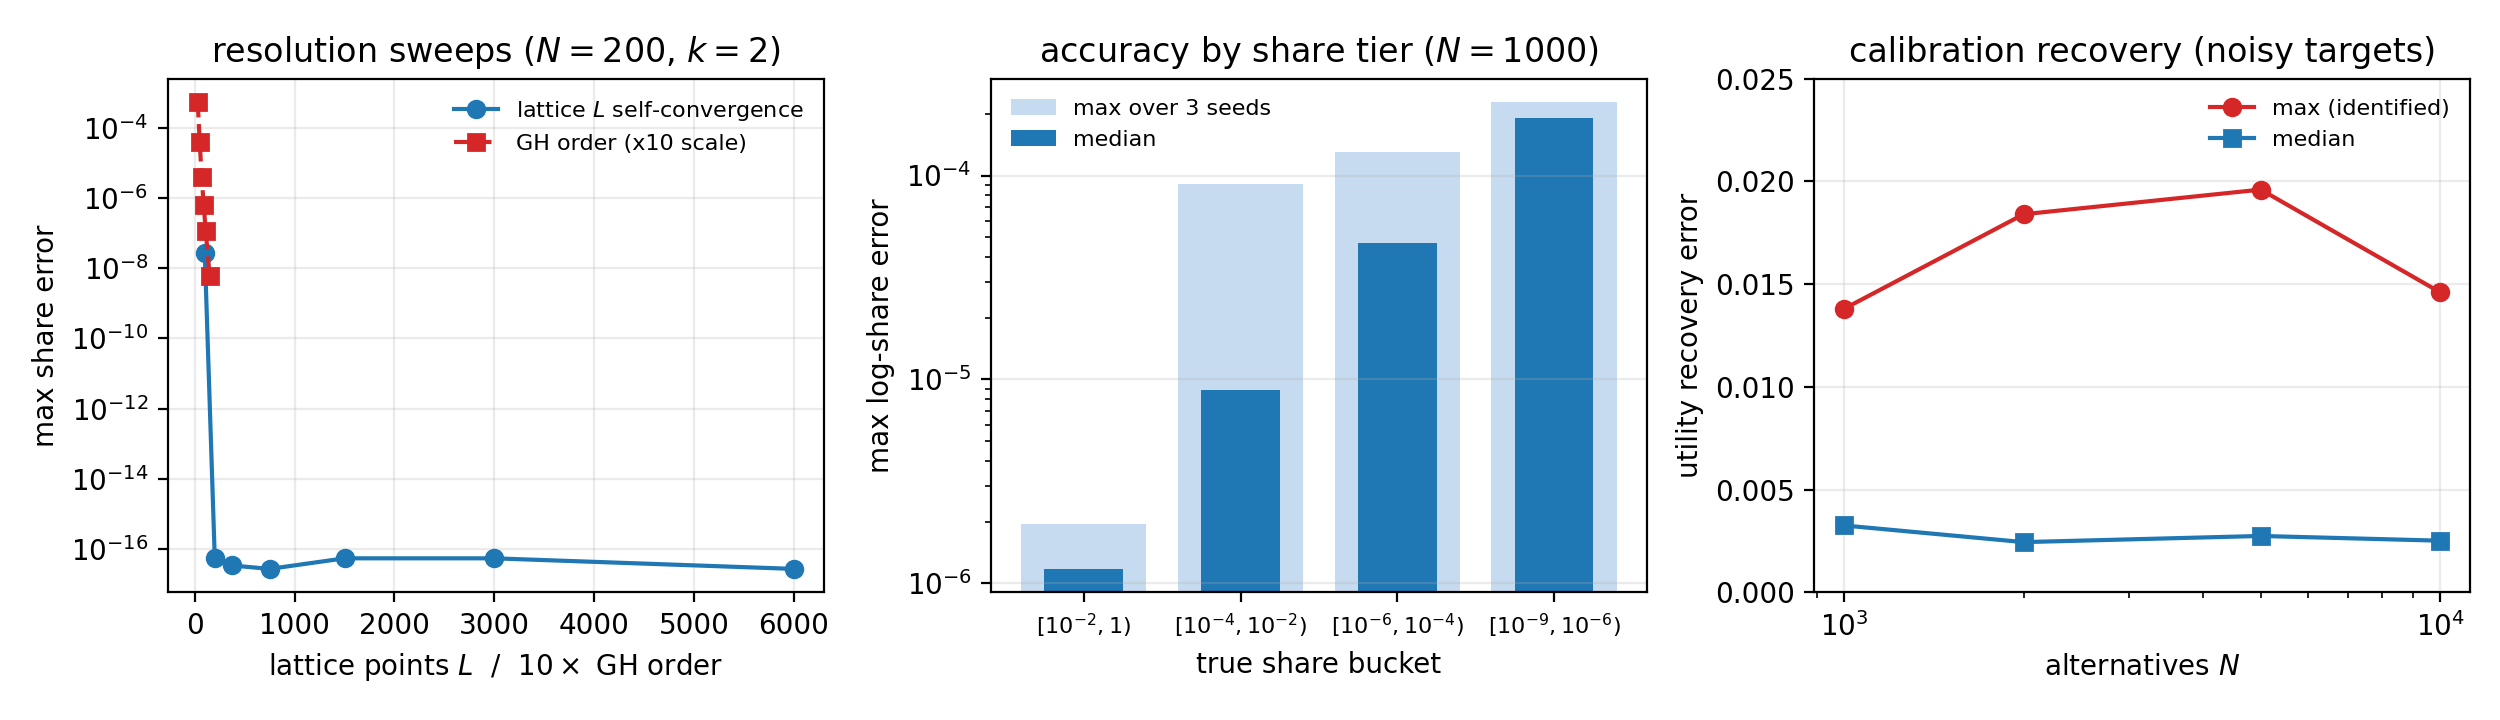
\includegraphics[width=\textwidth]{figs/validation.png}
\caption{Central validation evidence, from the committed experiments.
Left: lattice self-convergence in $L$ and Gauss--Hermite factor sweep
(experiment 17). Middle: log-share error against super-converged
references by true-share bucket at $N = 1000$, three problems
(experiment 25). Right: utility recovery against independent
$5\times10^6$-draw noisy targets over $N = 1000$ to $10000$
(experiment 19); the plateau is target sampling noise, not solver error
(experiment 21).}
\label{fig:validation}
\end{figure}

\paragraph{Resolution sweeps.} Figure~\ref{fig:validation} collects the
central accuracy evidence. Experiment 17 sweeps
each resolution knob separately at $N=200$, $k=2$.
Holding the factor rule fixed, lattice self-convergence is
$2.7\times10^{-8}$ at $L=101$ and at machine precision from $L \approx
200$; the convergence observed over the tested range is near-exponential,
and for these analytic, rapidly decaying integrands the lattice error
becomes negligible very quickly, leaving the $L$-error subdominant.

Holding $L$
fixed, the Gauss--Hermite sweep decays from $5.3\times10^{-4}$ (order 3) to
$5.9\times10^{-9}$ (order 15).

The pre-normalization defect
$|1 - \mathbf{1}^\top \tilde p\,|$ is $2.4\times10^{-8}$.

\paragraph{The price of smoothness.} Smoothness was never a side
issue in this literature; it shaped it. The raw frequency simulator is a
step function of the parameters, so \citet{stern1992} accepted a large
per-draw cost purely to smooth it, and GHK's adoption owed as much to
producing smooth, positive, differentiable estimates
\citep{hajivassiliou1998} as to its variance reduction. The lattice ends
that trade: it is smooth to resolution, and its derivatives are exact
integrals of the same pass, so the property the simulation literature
paid variance and wall time for costs nothing here.

\paragraph{Derivatives.} For fixed factor nodes and a fixed
lattice, the transform is a reproducible, (piecewise-)differentiable function
of $\mu$ whose derivatives are evaluated without resampling; analytic
own-location slopes of the unnormalized map come from the same pass and serve
as the inversion preconditioner. Along a utility path at $N=50$, the maximum second difference over $dt^2$
is 39.3 for fresh-draw GHK against 0.01 for both CRN-GHK and the lattice;
the committed smoothness figure shows the curves.

These are derivatives of the numerical
approximation, not exact MNP derivatives, and GHK-based practice likewise
differentiates its approximation, analytically or with fixed draws
\citep{hmr1996,hajivassiliou1998,train2009}. The practical distinction is the character and controllability of the
approximation error, quadrature resolution versus draw count, not the
possibility of differentiation.

\section{Calibration at $N=1000$}\label{sec:calibration}

At $N=1000$, $k=2$, with targets from
$5\times10^6$ MC draws floored at $10^{-7}$ and renormalized: the inversion
completes in 3 seconds compiled, 19 in the reference NumPy implementation
(all subsequent unlabeled timings are NumPy). The iteration solves its own equations to
$6.4\times10^{-9}$ (a statement about the solver, not statistical accuracy,
since the target carries sampling noise near $2\times10^{-4}$) and
recovers the utilities of the well-resolved alternatives (target share
above $3\times10^{-4}$) to maximum error $0.017$.

A replication study (experiment
16) repeats the inversion on a second $N=1000$ problem against three
independent $5\times10^6$-draw targets: 18 NumPy seconds each, 161--162
alternatives well-resolved (98.1\% of share mass), recovery error maximum
$0.015$--$0.023$ and median $\approx 0.0027$ across replicates, with the
recovery-versus-share curve committed alongside.

\paragraph{Validation: where the error comes from.} Experiment 21
separates the error sources. A noiseless inverse
test (targets generated by the lattice map itself, a deliberate inverse
crime that isolates solver plumbing) recovers the utilities of every
resolvable alternative to $6.5\times10^{-7}$ at $N=200$ and
$1.2\times10^{-7}$ at $N=1000$ --- solver error at the tolerance, so the
$\approx 0.02$ recovery in noisy tests is target sampling noise, not
solver error. Alternatives with shares below the resolution floor are not
chased, by design; their tier is reported separately.

\paragraph{Robustness.} Twenty problems that vary utility spread, factor
strength, $D$-heterogeneity, and rank all converged (6--31 iterations, recovery
$0.004$--$0.024$).

Numerical well-posedness matches
Proposition~\ref{thm:inv}: the reduced Jacobian assembled from $N$ JVP calls
at $N=50$ is symmetric to $1.7\times10^{-18}$, has row-sum defect
$6.2\times10^{-17}$, and reduced eigenvalues in $[2.5\times10^{-5},
0.22]$, positive definite as proved.

\paragraph{The error budget, by status.} Rigorous bounds and empirical
convergence evidence are different things, and the sources separate
cleanly:

\begin{center}
\footnotesize
\begin{tabular}{lp{6.2cm}}
\toprule
error source & status \\
\midrule
factor-node pruning & rigorous bound ($\delta$ sup-norm) \\
finite envelope & rigorous bound ($N\Phi(-8)$) \\
covariance approximation & rigorous KL/Pinsker bound (Section~\ref{sec:boundary}) \\
$x$-grid discretization & empirical convergence assessment \\
factor quadrature & empirical higher-order comparison \\
calibration residual & directly measured solver consistency \\
\bottomrule
\end{tabular}
\end{center}

\paragraph{Stability checks and two genuine bounds.} Self-convergence
checks at large $N$ show stability below what the
simulation references can resolve: refining to $(L = 3001, \mathrm{GH}21)$
moves the shares by $1.2\times10^{-8}$ at $N=1000$ and
$5.7\times10^{-8}$ at $N=5000$ (a stability statement, not by itself an
error bound, since both resolutions could share bias).

Two genuine bounds
come free from the product structure: conditional probabilities lie in
$[0,1]$, so pruning factor weight $\delta$ perturbs unnormalized shares by
at most $\delta = 2.39\times10^{-8}$ in sup norm (measured:
$6.2\times10^{-9}$); and the $\pm8\sigma_{\max}$ envelope omits
conditional mass at most $N\Phi(-8) + \Phi(-8)^N \le (N+1)\Phi(-8)
\approx 6\times10^{-12}$ even at $N = 10^4$ (the lower tail by a union
bound, the upper by independence).

\paragraph{Compiled implementation.} The same pass in Rust (in the
repository, with machine-precision parity and identical iteration counts)
calibrates $N=1000$ in 3 seconds, $N=5000$ in 18 seconds, and
$N=10000$ in 38 seconds (10, 11, and 13 iterations; independent
$5\times10^6$-draw targets, experiment 19).

\paragraph{Scaling.} Approximately linear in $N$ over the tested range
(experiment
19; at fixed spatial resolution the lattice would grow with the utility
range, $O(\sqrt{\log N})$ under Gaussian utilities): NumPy calibration
takes 16, 41, 110, and 201 seconds at $N = 1000$, $2000$, $5000$,
$10000$, a
flat 11--15
forward-pass equivalents throughout, with recovery quality unchanged
(median error near $0.003$, 96--99\% of share mass identified).

\paragraph{Why simulation cannot follow.} The gap here is structural,
and simple arithmetic shows why
(a plain independent Monte Carlo sample-complexity calculation, not a
lower bound on simulation methods generally). With common random numbers a
smoothed simulator such as CRN-GHK is a fixed function that a solver can
match to fine tolerance (a raw draw-and-argmax map is piecewise constant on
the $1/R$ grid and cannot be); either way the limitation is that it is the
wrong map.

Its coordinatewise error against the exact map is of order
$\sqrt{p_{\max}/R}$, so making the simulated map itself $\tau$-accurate
costs $R \approx p_{\max}/\tau^2$ independent draws per evaluation, and
inverting it exactly still leaves utilities whose true shares miss the
target at scale $\tau$, amplified through $J^{-1}$.

Under plain
independent direct simulation at the measured $N = 5000$ throughput, this
prices a forward map resolving the \emph{exact} MNP map to $\tau \sim
10^{-6}$ (this solver's model-consistency level, well beyond the
$2\times10^{-4}$ statistical accuracy of the noisy-target experiments) at
weeks per evaluation and the calibration in months to a year,
against seconds here: roughly six orders of magnitude, for this plain
direct-Monte-Carlo benchmark at the stated accuracy and measured
throughput.

Common
random numbers do not change the plain-MC rate, and randomized QMC and
specialized Gaussian integration can improve rates as well as
constants. The structural gap is different: per-alternative
formulations price $N$ separate integrals whose integrands each carry
$O(N)$ factors, and the shared field removes that factor of $N$. A
maximum over $N$ coordinates adds a further $\log N$ factor in
high-probability statements.

At the crude $\tau = 10^{-4}$ where
simulation-in-the-loop first becomes feasible, the calibrated model's true
shares miss the target at $10^{-4}$ and the answer moves with the draw
set.

The quadrature route's accuracy against the exact map is set by
resolution, not draws, at cost independent of $\tau$ until resolution
binds. We are unaware of a reported
probit share inversion at this scale in simulation-based practice, and this
scaling is presumably why.

\paragraph{Estimation gradients (by-product).} Experiment 30
parameterizes the covariance, $V(\theta) = \theta_1 V_0$ and
$D(\theta) = e^{\theta_2} D_0$, across four markets with known factor
scales, and differentiates a cross-market outer objective through the
calibration fixed point by the implicit function theorem, with the
reduced Newton solve built from Proposition~\ref{prop:jvp}'s
Jacobian--vector products. The implicit gradient matches central finite
differences to $1.2\times10^{-7}$, and a damped Newton outer loop
converges in three iterations --- to the truth up to the probit scale
gauge (recovered $\theta_1^2 e^{-\theta_2} = 1.000002$ against $1$),
which shares cannot identify. The scale ambiguity emerges from the
experiment rather than being imposed, and the machinery for the
differentiable estimation route of the discussion is thereby validated.

\paragraph{Removal ensemble (by-product).} The cached field also yields
all $N$ single-removal share vectors in $O(QN^2L)$: 15.9 seconds for all
200 removals at $N=200$, against 56.8 seconds recomputing.

Against the strongest simulation comparator, which reuses each draw's
winner and runner-up to answer every removal at once in $O(RN + N^2)$, the
deterministic ensemble is about $4.5\times$ more accurate at matched wall
time at $N=200$ ($4.2\times10^{-5}$ versus $1.9\times10^{-4}$;
experiment 18). This is a
side capability, not the paper's case.

\section{Boundary experiments}\label{sec:boundary}

\paragraph{General covariance through the factor approximation.} The method
requires $\Sigma \approx VV^\top + \mathrm{diag}(D)$; GHK does not. Choices depend on
$(\mu, \Sigma)$ only through $P\mu$ and $P\Sigma P$, $P = I -
\mathbf{1}\mathbf{1}^\top/N$, because the argmax is determined by
pairwise differences: a common factor loading $V \to V +
\mathbf{1}c^\top$ shifts every conditional location equally and cannot move
the argmax (a machine-precision identity), so the factor fit must be run in
this choice-relevant quotient space.

Fitting raw $\Sigma$ can spend
scarce rank on an irrelevant common component ($\Sigma = \tau^2
\mathbf{1}\mathbf{1}^\top + \beta\beta^\top + D$ with large $\tau$: the
raw rank-1 fit takes $\mathbf{1}\mathbf{1}^\top$ and misses
$\beta\beta^\top$ entirely; on such an example the contrast-space fit cuts
rank-1 share error from $4.6\times10^{-2}$ to $8.3\times10^{-3}$).

The
asymmetry matters: only the common \emph{factor} direction is irrelevant; a
common addition to $D$ inflates every difference variance and is
choice-relevant, so $D$ must come from the quotient fit.

The fit itself is
an iterative principal-factor heuristic applied to $P\Sigma P$ (eigendecompose
$P\Sigma P - \mathrm{diag}(D)$, take the top $k$ directions, refit $D$ from
the diagonal with a $10^{-3}$ floor, iterate to $10^{-10}$), followed by
centering and SVD canonicalization of the loadings (ordered columns, fixed
signs).

It is not certified to minimize a projected norm ($P\,\mathrm{diag}(D)\,P$
is not diagonal), so the repository also implements an alternating least-squares fit with
exact block updates on the reduced quotient (top-$k$ PSD step for the
loadings, nonnegative least squares for $D$; exact block minimization, not
a global-optimality certificate): on the boundary matrices it changes the
quotient residual by under 1\%, so the heuristic is not the binding
constraint.

The covariance-quotient residual $\|P(\Sigma -
\hat\Sigma)P\|_F / \|P\Sigma P\|_F$ is reported alongside every share
error in the committed output.

With this fit: correlation matrices at spectral decay $\lambda_m \propto
m^{-\gamma}$, $\gamma \in \{0.5, 1.5, 3\}$, at $N=50$, sharing one
orthogonal eigenbasis across $\gamma$ so decay comparisons are not
confounded with basis realization. The power law holds before diagonal
standardization, which perturbs the spectrum; the actual leading eigenvalues
(3.7, 17.1, 34.2 at $\gamma = 0.5, 1.5, 3$) are printed by the script.

Share error is measured against an $8\times10^6$-draw reference, with GHK
at the exact $\Sigma$ for comparison; the plotted quantity is the rank-$k$
approximation error of the stated procedure, not a minimum over factor
models.

Rank-8 errors: $1.8\times10^{-3}$, $3.7\times10^{-3}$, and
$3.1\times10^{-3}$ at $\gamma = 0.5, 1.5, 3$ from $k=1$ starting points of
$2.3\times10^{-3}$, $1.5\times10^{-2}$, $7.1\times10^{-2}$.

Decomposing the error with a second simulation under the fitted factor model:
lattice-versus-simulation discrepancy (which includes the finite
reference's own noise) is flat at $2$--$7\times10^{-4}$ across every $(\gamma,
k)$ tested, so the rank-$k$ error is essentially covariance-fit error:
rank, not quadrature, is the binding constraint.

Against GHK at $R = 10^4$
($3.2$, $2.3$, $4.3\times10^{-3}$), rank-8 wins at $\gamma = 0.5$ and $3$
but \emph{loses at intermediate decay} $\gamma = 1.5$
($3.7\times10^{-3}$ versus $2.3\times10^{-3}$): for this construction the
intermediate case is empirically hardest. Diagonal standardization perturbs
the nominal power law and the leading eigenvalue varies from 3.7 to 34.2
across the three cases, so this is not a clean one-parameter family.

Replication over three independent eigenbases: rank-8 beats GHK at $R=10^4$
in 8 of 9 basis--decay cases, with the single loss at intermediate decay.
The intermediate construction is empirically hardest, but this is not a
stable GHK-wins regime.

Nor is this wall-time-matched: the $k=8$ RQMC evaluation takes
15--24 s against 0.5--0.9 s for GHK at $R=10^4$, so at $N=50$ GHK is the
cheaper route to $3$--$4\times10^{-3}$; the lattice's advantage is large
$N$ at small $k$. Where accuracy demands exceed the achievable rank-$k$
error, GHK's arbitrary-$\Sigma$ generality is the right tool.

\paragraph{A certificate for the fit.} Winner events depend only on
contrasts, so for any basis $B$ of $\mathbf{1}^\perp$, Pinsker's
inequality bounds every share discrepancy by the Kullback--Leibler
divergence between the contrast Gaussians:
\[
|p_i(\Sigma) - p_i(\hat\Sigma)| \le
\sqrt{\tfrac12\,\mathrm{KL}\big(\mathcal{N}(B^\top\mu, B^\top\Sigma B)\,\|\,
\mathcal{N}(B^\top\mu, B^\top\hat\Sigma B)\big)},
\]
with the Gaussian KL in closed form. Measured (experiment 26), the bound is roughly two
orders of magnitude conservative but informative exactly where
certification matters: fitting two factors to a fast-decaying
four-factor truth certifies share error below $5.3\times10^{-2}$
(actual $4\times10^{-4}$), and three factors certify
$8.4\times10^{-3}$ (actual $9.7\times10^{-5}$). It converts the fitted pair of contrast covariances, through their
Gaussian KL divergence, into a hard share-error guarantee before any
transform is run.

\paragraph{Substitution: a $2\times2$ factorial illustration.} The design varies factor
structure and noise family one axis at a time (with a caveat below),
holding the idiosyncratic
scale common. Coupling either axis with alternative-specific scales would
confound the comparison: an alternative-specific-scale Gumbel race is not
mixed logit, and heteroskedasticity alone already breaks IIA. One
confound must be named: the factor loadings $v_{ir} \sim N(0, 0.36/k)$
add $\|v_i\|^2$ to each marginal variance, unevenly across
alternatives, so the factor axis changes marginal scales as well as
covariance; it is more precisely a \emph{full factor covariance} axis.
The equal-marginal-variance replication (experiment 29) repairs this:
loadings normalized to $\|v_i\|^2 = 0.36$, idiosyncratic variance
$0.64$, so every marginal is exactly one and the axis moves only the
off-diagonal covariance; twenty seeds, independent $5\times10^6$-draw
targets. The pure-covariance effect is larger, not smaller: median
misallocation of released demand (logit against factor probit) is
$0.245$ against $0.009$ for deleted shares above ten percent,
$0.275$ against $0.031$ at 2--10\%, and $0.325$ against $0.113$ at
0.5--2\%, with factor probit winning all twenty paired seeds in each of
those strata; below $0.5\%$ both degrade ($0.78$ against $0.68$, 17 of
20) as the targets' resolution binds.

Ground truth ($N = 50$) is misspecified for every candidate: $t(5)$ factors
(unit variance) and skew-normal idiosyncratic noise (shape $a = 3$),
standardized to mean zero and unit variance, homoskedastic, with $\mu^\star
\sim N(0,1)$ and oracle loadings $v^\star_{ir} \sim N(0, 0.36/k)$, $k=2$.
(The race is computed min-wins, so positive skew in race coordinates is
\emph{left}-skew in utility coordinates.)

The four candidates hold the idiosyncratic scale fixed and vary
$\{\text{Gumbel}, \text{Gaussian}\}$ base $\times$ $\{V = 0, V =
V^\star\}$. The Gumbel base is variance-standardized to one, so the
family axis does not alter the factor-to-idiosyncratic variance ratio.

Because the implementation is min-wins, the Gumbel base is the
\emph{reflected} (minimum) Gumbel corresponding to a standard
maximum-Gumbel in utility coordinates; the committed anchor verifies that
its zero-loading case equals softmax at $N=12$ to $2.8\times10^{-17}$.
The candidate factor law is Gaussian in all cases, so the truth's $t(5)$
factor law is misspecified for every candidate.

This is an \emph{oracle-loading} design: both factor
candidates receive the true $V^\star$ rather than estimating it. All four
are calibrated to the same full-menu shares (residuals $\le
4\times10^{-10}$).

Deletion truths come from $2\times10^7$ \emph{common} utility draws with
the top three alternatives retained per draw, from which every
single-deletion and pair-deletion truth follows with common random numbers.

Of 150 deletion blocks (50 singles, 100 fixed-seed random pairs), 45 with
deleted mass below 0.05\% are excluded as unresolvable; of the 105 scored
blocks, 83 fall in the three best-resolved strata (26/29/28 at $>$10\% /
2--10\% / 0.5--2\%) and the remaining 22, with deleted mass between
0.05\% and 0.5\%, appear in the final column (their truths sit closest to
the common-draw resolution floor, so that column carries the widest error
bars).

The score per deletion block $B$ is the
misallocated fraction of the redistributed mass,
\[
\mathrm{TV}\!\left(q^{(-B)}_{\mathrm{model}},\,
q^{(-B)}_{\mathrm{truth}}\right) \Big/ \textstyle\sum_{i \in B} p_i ,
\]
averaged within strata:

\begin{center}
\begin{tabular}{lcccc}
\toprule
 & mass $>10\%$ & 2--10\% & 0.5--2\% & 0.05--0.5\% \\
\midrule
independent Luce (= plain logit) & 0.229 & 0.245 & 0.261 & 0.305 \\
independent probit & 0.210 & 0.232 & 0.230 & 0.267 \\
factor mixed logit & 0.114 & 0.146 & 0.199 & 0.244 \\
factor probit & \textbf{0.045} & \textbf{0.062} & \textbf{0.094} & \textbf{0.116} \\
\bottomrule
\end{tabular}
\end{center}

The factorial decomposition (top two strata): the factor increment is
dominant in both families ($+0.115/+0.099$ within Gumbel, $+0.165/+0.170$
within Gaussian); the family increment alone is small ($+0.019/+0.013$ at $V
= 0$) but grows with factors present ($+0.069/+0.084$), a negative
interaction ($-0.050/-0.071$): factor structure and the Gaussian base are
complements in this design.

Caveats: a single truth design and seed, and a skew-normal truth that is
Gaussian-adjacent. The figure plots, for each scored single deletion, plain
logit's misallocation against factor probit's: points below the diagonal
are deletions where factor probit is closer to the truth. Singles and pairs
score similarly (factor probit 0.080 versus 0.076 mean misallocated
fraction) and are summarized separately in the committed output.

\begin{figure}[h]
\centering

\includegraphics[width=0.48\textwidth]{figs/full_sigma.png}\hfill
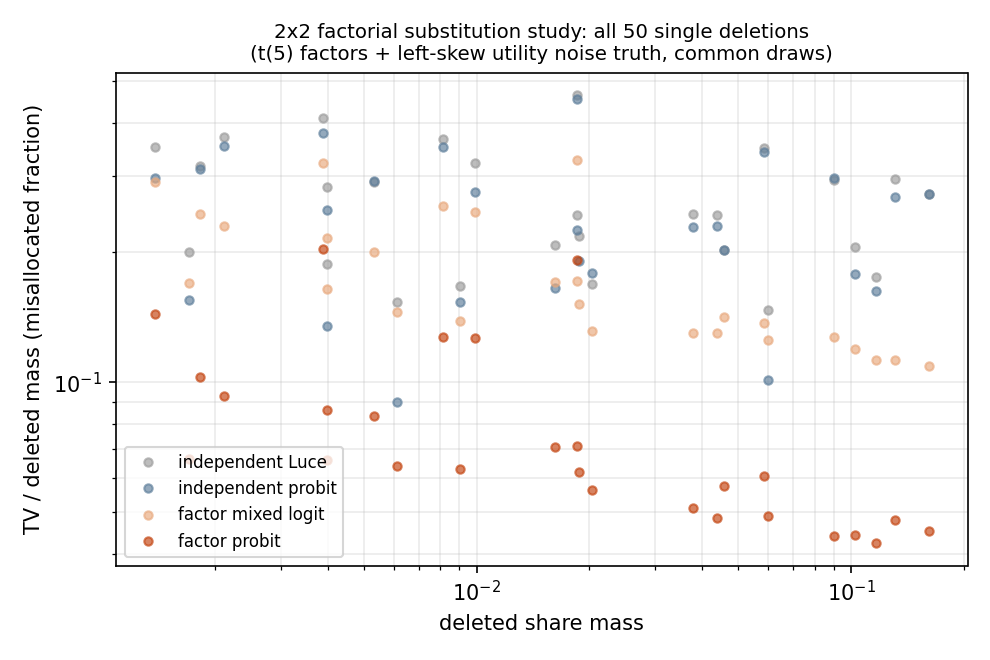
\includegraphics[width=0.48\textwidth]{figs/factorial.png}
\caption{Left: rank-$k$ contrast-space approximation error under spectral
decay $\gamma$ (dotted: GHK at $R=10^4$, per $\gamma$; not wall-time
matched). Right: paired comparison on identical deletions --- plain
logit's misallocated fraction (horizontal) against factor probit's
(vertical), one point per scored single deletion, shaded by deleted mass;
the dashed line is parity.}
\label{fig:boundary}
\end{figure}

\section{Related work}\label{sec:related}

GHK and simulated likelihood are standard in econometrics
\citep{geweke1994,hajivassiliou1998,train2009}, with
\citet{hmr1996} the standard treatment of simulated MVN probabilities
and their derivatives; \citet{genz1992}
developed the same separation-of-variables construction in numerical
statistics, where its RQMC form is the default MVN evaluator, anchored
by the Genz--Bretz book \citep{genzbretz2009} and the \texttt{mvtnorm}
package \citep{mi2009}.

Deterministic grid recursions exist within that ecosystem: \citet{miwa2003}
evaluate orthant probabilities by recursion on one-dimensional lattices,
at factorial cost in the dimension for general correlation, and
\citet{craig2008} accelerates the Markov case; both price one
probability per run. \citet{ridgway2016} reads GHK as sequential importance sampling, proves its
variance can deteriorate exponentially, and builds SMC alternatives; \citet{botev2017} sharpened the family with minimax tilting;
\citet{genton2018} began the hierarchical line in this journal;
\citet{cao2021} push MVN probabilities to thousands of
dimensions with tile-low-rank QMC, machinery pointed almost exactly at our
difference covariances, which are diagonal plus rank $k+1$; and
\citet{cao2025} reach linear per-probability cost past twenty thousand
dimensions with Vecchia approximations.

Deterministic approximations run from Mendell--Elston \citep{mendell1974}
(surprisingly competitive when optimally ordered \citep{connors2014})
through Bhat's MACML \citep{bhat2011} to expectation propagation:
\citet{cunningham2011} found EP
highly accurate precisely for rectangular regions, and \citet{fasano2025} evaluate generic Gaussian CDFs by EP on a dual probit
model, deterministically and sampling-free. Every one of these prices one
orthant at a time; none couples the $N$ winner probabilities.

Factor dimension reduction for probit is old, and older than
econometrics: \citet{curnow1962} showed that product correlation
collapses the multivariate normal integral to a one-dimensional integral
of products of univariate CDFs, the reduction this paper conditions on,
and \citet{dunnett1989} is its standard algorithm. The ranking-and-selection
tradition built on the same integrals from the 1950s
\citep{bechhofer1954,gupta1963}, always evaluating one designated
candidate per integral: assembling all $N$ that way costs $N$ separate
integrals where the shared field gives all $N$ in one pass.

In
econometrics, \citet{butler1982} integrated one factor by quadrature;
\citet{mcfadden1984} proposed factor-analytic MNP expressly as dimension
reduction; \citet{stern1992} used the same conditional-independence
product of normal CDFs with Monte Carlo over the residual;
\citet{bolduc1999} handled large choice sets with parsimonious
covariances but simulated probabilities.

\citet{elrod1995}
estimated factor-analytic probit for panel data;
\citet{loaiza2022} pursue large choice sets by
Bayesian estimation, with variational follow-ups \citep{loaiza2023};
\citet{kim2026} reach twenty alternatives at a million observations by
neural variational inference, and \citet{ding2024} exceed a hundred with
expectation-propagation E-steps. All are approximate forward maps for
estimation; none inverts shares. \citet{girolami2006} use the
one-dimensional product identity in its diagonal-covariance form,
per class. \citet{collier2021} place the factor-Gaussian race with
low-rank-plus-diagonal covariance on the last layer of large-scale image
classifiers, including thousand-class ImageNet, and approximate the
winner probabilities by Monte Carlo over a temperature-softmax
relaxation; \citet{berthet2020} differentiate general perturbed-argmax
layers by Monte Carlo, with $p = \nabla G$ as the organizing identity.
Both simulate the map this paper evaluates deterministically. The racing literature posed both
ingredients first: \citet{henery1981} wrote the survival-product win
integral for normal running times and gave its first-order analytic
inversion, \citet{ali1998} inverted market odds to abilities numerically
at eight-runner fields, and betting practice otherwise approximated the
inversion away \citep{lo1994}. The lattice survival-product identity and
its fast inverse transform come from racing \citep{cotton2021}, which
names the common-factor extension developed here as an open problem.

The shared-product assembly itself also appears in competing-risks
computation: \citet{mahani2019} compute all cause-specific cumulative
incidences on one shared grid by forming the product of every survival
function once and dividing out each cause's own factor (software since
2015), and the Aalen--Johansen estimator \citep{aalen1978} reads all
causes off a single survival product nonparametrically. Neither embeds
the assembly in factor quadrature, differentiates it, nor inverts it;
racing arrived at it independently.

Conditioning on the factors and the alternative's own shock makes each
probability a $(k{+}1)$-dimensional integral,
\[
p_i = \E_{f,z} \prod_{j \ne i}
\Phi\!\left(\frac{\mu_i - \mu_j + (v_i - v_j)^\top f +
\sqrt{D_i}\,z}{\sqrt{D_j}}\right),
\]
evaluable per alternative by modern randomized quasi-Monte Carlo: the
natural competitor that uses exactly the structure this paper assumes. It
still prices $N$ separate integrals, $O(RN^2)$ in total, where the shared
field couples them into one $O(QN(k+L))$ pass. Measured at matched
$4\times10^{-4}$ accuracy (experiment 24; the two implementations first
verified against each other to $1.7\times10^{-5}$), the per-alternative
route needs 215 seconds at $N = 1000$ against the shared field's 1.5,
a gap of $140\times$ that widens linearly in $N$.

An older transportation literature used ``calibration'' for MNP
parameter estimation. \citet{daganzo1977} introduced an early numerical
MNP forecasting algorithm and claimed applicability to large problems;
\citet{sheffi1982} reviewed probability and calibration methods and
proposed simulation-based estimation; \citet{kamakura1989} embedded the
Mendell--Elston approximation in a calibration routine. These estimate
parameters from choice data or approximate designated probabilities;
none provides a smooth all-$N$ share map, a shared-field
Jacobian--vector product, or aggregate-share inversion at the scale
considered here.

Inversion theory is likewise established. \citet{berry1994} made
share-to-utility inversion the workhorse of demand estimation;
\citet{bonnet2022} invert demand in general, including nonsmooth
random-utility models, through two-sided matching;
\citet{hotz1993}
inverted choice probabilities to utility differences; \citet{norets2013}
prove surjectivity of the utility-to-probability map;
\citet{bgh2013} obtain demand invertibility from
connected substitution;
\citet{chiong2016} invert through the convex
conjugate; \citet{fosgerau2020} show the probit inverse exists by
generalized-entropy duality, without an algorithm.

 \citet{berry1995} built demand
estimation on the logit-side inversion, and \citet{conlon2020}
maintain its modern practice. \citet{chia2021}
differentiates logit BLP automatically; \citet{huch2026}
amortize correlated-choice probabilities with neural networks, evidence of
current demand for this computation.

The novelty here is accordingly none of: dimension reduction
\citep{curnow1962}, the order-statistic integral, the shared-product
assembly in isolation \citep{mahani2019,cotton2021}, or well-posedness of
inversion. It is the
all-alternatives assembly in $O(QNL)$, its large-$N$ implementation, the
$O(QNL)$ Jacobian--vector product, and the shared-field reuse for
calibration and counterfactuals.

\section{Discussion}\label{sec:discussion}

Estimation is the natural next step. With the reduced coordinates of
Proposition~\ref{prop:ident}, gradients of an outer likelihood or GMM
objective pass through the calibration fixed point by implicit
differentiation, a route to differentiable probit demand estimation at large
$N$. Estimating $(V, D)$ rather than supplying them raises the usual
identification cautions: scale normalization, factor rotation, and the fact
that only difference covariances are identified.

The pass itself can be accelerated further: its two stages are smooth-kernel
sums whose matrices are numerically low-rank, and a Chebyshev-separated
evaluation (in the spirit of black-box fast multipole methods) reduces
each node's cost from $O(NL)$ to $O(r(N+L))$, with exponential
convergence in $r$. A forward-map prototype is committed (experiment
20); its systematic error control and extension to the derivative and
calibration passes are developed in a companion paper.

Beyond the Gaussian family, the same machinery computes races with arbitrary
alternative-specific idiosyncratic densities. A common-scale Gumbel base with
zero loadings reproduces the Luce model exactly, yielding correlated-softmax
generalizations.

Neither method class dominates the other. Simulation owns arbitrary
$\Sigma$ and coarse accuracy; the shared field owns the factor form,
tight accuracy, derivatives, and calibration; the boundary experiments
illustrate that covariance approximation, rather than quadrature,
becomes the binding limitation when the choice-relevant covariance is
not well represented at modest rank. We leave to future work
replication of the substitution factorial across truth designs and a
walk-forward calibration on real assortment data.

For fifty years, computability decided which choice models get used. For
the factor form of probit, the form in which correlated utilities entered
econometrics \citep{hausman1978}, that constraint is gone: all shares, Jacobian--vector products, and
the inverse map cost seconds at ten thousand alternatives. Integrating
factor estimation with this inner solver is outside the present paper,
and with $(V, D)$ in hand the choice
between logit and probit families becomes one of fit, not tractability.

\section*{Reproducibility and Supplementary Materials}

\begin{description}
\item[Code and experiments:] all numbers come from committed, seeded
scripts with correctness anchors run before any comparison (repository
experiments 13--26 and 29--31; 27 and 28 support the companion paper).
A single manifest,
\texttt{experiments/run\_all\_paper.py}, regenerates every table and
figure; this submission is built from the immutable tag
\texttt{jcgs-v1}. (Archive supplied as a zip with
the submission; development repository at
\url{https://github.com/microprediction/kinetics}.)
\item[Software:] the algorithm ships in an open-source Python package
with an optional compiled (Rust) kernel, and package--benchmark agreement
is itself a reported number.
\item[Data:] all experiments use synthetic data generated by the seeded
scripts; no external data are required.
\end{description}

Hardware and software: Apple M4, 16\,GB, Python 3.12.9,
NumPy 2.4.6, SciPy 1.18.0; compiled timings use rustc 1.97.1
(release profile, rayon defaulting to all performance cores); experiment 17 enforces single-threaded BLAS via
\texttt{threadpoolctl}; sub-second timings are warmed medians of three
runs, and long simulations are single realizations, disclosed as such.
Monte Carlo chunk sizes derive from an explicit 1.5\,GB memory budget, and
peak resident memory stays below 2\,GB.

\section*{Disclosure Statement}

The author reports no conflicts of interest. No external funding was
received for this work.

\begin{thebibliography}{9}
\bibitem[Williams(1977)]{williams1977} H.~C.~W.~L. Williams. On the
formation of travel demand models and economic evaluation measures of
user benefit. \emph{Environment and Planning A} 9 (1977) 285--344.

\bibitem[Daly and Zachary(1978)]{daly1978} A.~Daly, S.~Zachary.
Improved multiple choice models. In D.~Hensher, M.~Dalvi (eds.),
\emph{Determinants of Travel Choice}, Saxon House, 1978.

\bibitem[Lazear and Rosen(1981)]{lazear1981} E.~P. Lazear, S.~Rosen.
Rank-order tournaments as optimum labor contracts. \emph{Journal of
Political Economy} 89 (1981) 841--864.

\bibitem[Mosteller(1951)]{mosteller1951} F.~Mosteller. Remarks on the
method of paired comparisons I. \emph{Psychometrika} 16 (1951) 3--9.

\bibitem[Daganzo et~al.(1977)Daganzo, Bouthelier, and
Sheffi]{daganzo1977} C.~F. Daganzo, F.~Bouthelier, Y.~Sheffi.
Multinomial probit and qualitative choice: a computationally efficient
algorithm. \emph{Transportation Science} 11 (1977) 338--358.

\bibitem[Sheffi et~al.(1982)Sheffi, Hall, and Daganzo]{sheffi1982}
Y.~Sheffi, R.~Hall, C.~F. Daganzo. On the estimation of the multinomial
probit model. \emph{Transportation Research Part A} 16 (1982) 447--456.

\bibitem[Kamakura(1989)]{kamakura1989} W.~A. Kamakura. The estimation
of multinomial probit models: a new calibration algorithm.
\emph{Transportation Science} 23 (1989) 253--265.

\bibitem[Bonnet et~al.(2022)Bonnet, Galichon, Hsieh, O'Hara, and
Shum]{bonnet2022} O.~Bonnet, A.~Galichon, Y.-W. Hsieh, K.~O'Hara,
M.~Shum. Yogurts choose consumers? Estimation of random-utility models
via two-sided matching. \emph{Review of Economic Studies} 89 (2022)
3085--3114.

\bibitem[McFadden(1984)]{mcfadden1984} D.~McFadden. Econometric
analysis of qualitative response models. In Z.~Griliches,
M.~Intriligator (eds.), \emph{Handbook of Econometrics}, vol.~II,
North-Holland, 1984, 1395--1457.

\bibitem[Stern(1992)]{stern1992} S.~Stern. A method for smoothing
simulated moments of discrete probabilities in multinomial probit
models. \emph{Econometrica} 60 (1992) 943--952.

\bibitem[Berry(1994)]{berry1994} S.~Berry. Estimating discrete-choice
models of product differentiation. \emph{RAND Journal of Economics} 25
(1994) 242--262.

\bibitem[Bolduc(1999)]{bolduc1999} D.~Bolduc. A practical technique to
estimate multinomial probit models in transportation. \emph{Transportation
Research B} 33 (1999) 63--79.

\bibitem[Hausman and Wise(1978)]{hausman1978} J.~A. Hausman, D.~A.
Wise. A conditional probit model for qualitative choice: discrete
decisions recognizing interdependence and heterogeneous preferences.
\emph{Econometrica} 46 (1978) 403--426.

\bibitem[Thurstone(1927)]{thurstone1927} L.~L. Thurstone. A law of comparative judgment.
\emph{Psychological Review} 34 (1927) 273--286.
\bibitem[Geweke et~al.(1994)Geweke, Keane, and Runkle]{geweke1994} J.~Geweke, M.~Keane, D.~Runkle. Alternative computational
approaches to inference in the multinomial probit model. \emph{Review of
Economics and Statistics} 76 (1994) 609--632.
\bibitem[Hajivassiliou and McFadden(1998)]{hajivassiliou1998} V.~Hajivassiliou, D.~McFadden. The method of
simulated scores for the estimation of LDV models. \emph{Econometrica} 66
(1998) 863--896.
\bibitem[Train(2009)]{train2009} K.~Train. \emph{Discrete Choice Methods with Simulation},
2nd ed. Cambridge, 2009.
\bibitem[Henery(1981)]{henery1981} R.~J. Henery. Permutation
probabilities as models for horse races. \emph{Journal of the Royal
Statistical Society B} 43 (1981) 86--91.

\bibitem[Ali(1998)]{ali1998} M.~M. Ali. Probability models on horse-race
outcomes. \emph{Journal of Applied Statistics} 25 (1998) 221--229.

\bibitem[Lo and Bacon-Shone(1994)]{lo1994} V.~S.~Y. Lo, J.~Bacon-Shone.
A comparison between two models for predicting ordering probabilities in
multiple-entry competitions. \emph{The Statistician} 43 (1994) 317--327.

\bibitem[Loaiza-Maya and Nibbering(2023)]{loaiza2023} R.~Loaiza-Maya,
D.~Nibbering. Fast variational Bayes methods for multinomial probit
models. \emph{Journal of Business \& Economic Statistics} 41 (2023)
1352--1363.

\bibitem[Kim et~al.(2026)Kim, Kang, Kock, Bansal, and Sohn]{kim2026}
G.~Kim, Y.~Kang, L.~Kock, P.~Bansal, K.~Sohn. Scalable variational
inference for multinomial probit models under large choice sets and
sample sizes. \emph{Statistics and Computing} 36 (2026) 47.

\bibitem[Ding et~al.(2024)Ding, Imbens, Qu, and Ye]{ding2024} P.~Ding,
G.~Imbens, Z.~Qu, Y.~Ye. Computationally efficient estimation of large
probit models. arXiv:2407.09371 (2024).

\bibitem[Collier et~al.(2021)Collier, Mustafa, Kokiopoulou, Jenatton,
and Berent]{collier2021} M.~Collier, B.~Mustafa, E.~Kokiopoulou,
R.~Jenatton, J.~Berent. Correlated input-dependent label noise in
large-scale image classification. \emph{Proceedings of CVPR} (2021)
1551--1560.

\bibitem[Berthet et~al.(2020)Berthet, Blondel, Teboul, Cuturi, Vert, and
Bach]{berthet2020} Q.~Berthet, M.~Blondel, O.~Teboul, M.~Cuturi,
J.-P.~Vert, F.~Bach. Learning with differentiable perturbed optimizers.
\emph{Advances in Neural Information Processing Systems} 33 (2020)
9508--9519.

\bibitem[Girolami and Rogers(2006)]{girolami2006} M.~Girolami,
S.~Rogers. Variational Bayesian multinomial probit regression with
Gaussian process priors. \emph{Neural Computation} 18 (2006) 1790--1817.

\bibitem[Fosgerau et~al.(2020)Fosgerau, Melo, de~Palma, and
Shum]{fosgerau2020} M.~Fosgerau, E.~Melo, A.~de~Palma, M.~Shum. Discrete
choice and rational inattention: a general equivalence result.
\emph{International Economic Review} 61 (2020) 1569--1589.

\bibitem[Mahani and Sharabiani(2019)]{mahani2019} A.~S. Mahani,
M.~T.~A. Sharabiani. Bayesian, and non-Bayesian, cause-specific
competing-risk analysis for parametric and nonparametric survival
functions: the R package CFC. \emph{Journal of Statistical Software} 89
(2019) 1--29.

\bibitem[Aalen and Johansen(1978)]{aalen1978} O.~O. Aalen, S.~Johansen.
An empirical transition matrix for non-homogeneous Markov chains based on
censored observations. \emph{Scandinavian Journal of Statistics} 5
(1978) 141--150.

\bibitem[Curnow and Dunnett(1962)]{curnow1962} R.~N. Curnow, C.~W.
Dunnett. The numerical evaluation of certain multivariate normal
integrals. \emph{Annals of Mathematical Statistics} 33 (1962) 571--579.

\bibitem[Dunnett(1989)]{dunnett1989} C.~W. Dunnett. Algorithm AS 251:
multivariate normal probability integrals with product correlation
structure. \emph{Applied Statistics} 38 (1989) 564--579.

\bibitem[Bechhofer(1954)]{bechhofer1954} R.~E. Bechhofer. A single-sample
multiple decision procedure for ranking means of normal populations with
known variances. \emph{Annals of Mathematical Statistics} 25 (1954)
16--39.

\bibitem[Gupta(1963)]{gupta1963} S.~S. Gupta. Probability integrals of
multivariate normal and multivariate $t$. \emph{Annals of Mathematical
Statistics} 34 (1963) 792--828.

\bibitem[Butler and Moffitt(1982)]{butler1982} J.~S. Butler, R.~Moffitt. A computationally efficient
quadrature procedure for the one-factor multinomial probit model.
\emph{Econometrica} 50 (1982) 761--764.
\bibitem[Elrod and Keane(1995)]{elrod1995} T.~Elrod, M.~P. Keane. A factor-analytic probit model for
representing the market structure in panel data. \emph{Journal of Marketing
Research} 32 (1995) 1--16.
\bibitem[Bhat(2011)]{bhat2011} C.~Bhat. The maximum approximate composite marginal
likelihood (MACML) estimation of multinomial probit-based unordered response
choice models. \emph{Transportation Research B} 45 (2011) 923--939.
\bibitem[Connors et~al.(2014)Connors, Hess, and Daly]{connors2014} R.~Connors, S.~Hess, A.~Daly. Analytic approximations
for computing probit choice probabilities. \emph{Transportmetrica A} 10
(2014) 119--139.
\bibitem[Botev(2017)]{botev2017} Z.~Botev. The normal law under linear restrictions:
simulation and estimation via minimax tilting. \emph{JRSS-B} 79 (2017)
125--148.
\bibitem[Cotton(2021)]{cotton2021} P.~Cotton. Inferring relative ability from winning
probability in multientrant contests. \emph{SIAM J.\ Financial Mathematics}
12 (2021) 295--317.
\bibitem[Hotz and Miller(1993)]{hotz1993} V.~J. Hotz, R.~A. Miller. Conditional choice
probabilities and the estimation of dynamic models. \emph{Review of
Economic Studies} 60(3):497--529, 1993.

\bibitem[Berry et~al.(2013)Berry, Gandhi, and Haile]{bgh2013} S.~Berry, A.~Gandhi, P.~Haile. Connected substitutes
and invertibility of demand. \emph{Econometrica} 81(5):2087--2111, 2013.

\bibitem[Berry et~al.(1995)Berry, Levinsohn, and Pakes]{berry1995} S.~Berry, J.~Levinsohn, A.~Pakes. Automobile prices in
market equilibrium. \emph{Econometrica} 63 (1995) 841--890.
\bibitem[Conlon and Gortmaker(2020)]{conlon2020} C.~Conlon, J.~Gortmaker. Best practices for
differentiated products demand estimation with pyblp. \emph{RAND Journal of
Economics} 51 (2020) 1108--1161.
\bibitem[Chia(2021)]{chia2021} A.~Chia. Automatically differentiable random coefficient
logistic demand estimation. arXiv:2106.04636 (2021).
\bibitem[Huch and Keane(2026)]{huch2026} E.~Huch, M.~Keane. Amortized inference for correlated
discrete choice models via equivariant neural networks. arXiv:2603.24705
(2026).
\bibitem[McFadden(1981)]{mcfadden1981} D.~McFadden. Econometric models of probabilistic
choice. In C.~Manski, D.~McFadden (eds.), \emph{Structural Analysis of
Discrete Data}, MIT Press, 1981.
\bibitem[Chiong et~al.(2016)Chiong, Galichon, and Shum]{chiong2016} K.~Chiong, A.~Galichon, M.~Shum. Duality in dynamic
discrete-choice models. \emph{Quantitative Economics} 7 (2016) 83--115.
\bibitem[Norets and Takahashi(2013)]{norets2013} A.~Norets, S.~Takahashi. On the surjectivity of the
mapping between utilities and choice probabilities. \emph{Quantitative
Economics} 4 (2013) 149--155.
\bibitem[Loaiza-Maya and Nibbering(2022)]{loaiza2022} R.~Loaiza-Maya, D.~Nibbering. Scalable Bayesian
estimation in the multinomial probit model. \emph{Journal of Business \&
Economic Statistics} 40 (2022) 1678--1690.
\bibitem[Hajivassiliou et~al.(1996)Hajivassiliou, McFadden, and
Ruud]{hmr1996} V.~Hajivassiliou, D.~McFadden, P.~Ruud. Simulation of
multivariate normal rectangle probabilities and their derivatives:
theoretical and computational results. \emph{Journal of Econometrics} 72
(1996) 85--134.

\bibitem[Genz and Bretz(2009)]{genzbretz2009} A.~Genz, F.~Bretz.
\emph{Computation of Multivariate Normal and $t$ Probabilities}. Lecture
Notes in Statistics 195, Springer, 2009.

\bibitem[Mi et~al.(2009)Mi, Miwa, and Hothorn]{mi2009} X.~Mi, T.~Miwa,
T.~Hothorn. mvtnorm: new numerical algorithm for multivariate normal
probabilities. \emph{The R Journal} 1 (2009) 37--39.

\bibitem[Miwa et~al.(2003)Miwa, Hayter, and Kuriki]{miwa2003} T.~Miwa,
A.~J. Hayter, S.~Kuriki. The evaluation of general non-centred orthant
probabilities. \emph{Journal of the Royal Statistical Society B} 65
(2003) 223--234.

\bibitem[Craig(2008)]{craig2008} P.~Craig. A new reconstruction of
multivariate normal orthant probabilities. \emph{Journal of the Royal
Statistical Society B} 70 (2008) 227--243.

\bibitem[Genton et~al.(2018)Genton, Keyes, and Turkiyyah]{genton2018}
M.~G. Genton, D.~E. Keyes, G.~Turkiyyah. Hierarchical decompositions for
the computation of high-dimensional multivariate normal probabilities.
\emph{Journal of Computational and Graphical Statistics} 27 (2018)
268--277.

\bibitem[Cao and Katzfuss(2025)]{cao2025} J.~Cao, M.~Katzfuss.
Linear-cost Vecchia approximation of multivariate normal probabilities.
\emph{Journal of the American Statistical Association} 121 (2026)
768--781.

\bibitem[Genz(1992)]{genz1992} A.~Genz. Numerical computation of multivariate normal
probabilities. \emph{J.\ Computational and Graphical Statistics} 1 (1992)
141--149.
\bibitem[Ridgway(2016)]{ridgway2016} J.~Ridgway. Computation of Gaussian orthant
probabilities in high dimension. \emph{Statistics and Computing} 26 (2016)
899--916.
\bibitem[Cao et~al.(2021)Cao, Genton, Keyes, and Turkiyyah]{cao2021} J.~Cao, M.~G. Genton, D.~E. Keyes, G.~M. Turkiyyah.
Exploiting low-rank covariance structures for computing high-dimensional
normal and Student-$t$ probabilities. \emph{Statistics and Computing} 31
(2021) 2.
\bibitem[Mendell and Elston(1974)]{mendell1974} N.~R. Mendell, R.~C. Elston. Multifactorial
qualitative traits: genetic analysis and prediction of recurrence risks.
\emph{Biometrics} 30 (1974) 41--57.
\bibitem[Cunningham et~al.(2011)Cunningham, Hennig, and Lacoste-Julien]{cunningham2011} J.~P. Cunningham, P.~Hennig, S.~Lacoste-Julien.
Gaussian probabilities and expectation propagation. arXiv:1111.6832 (2011).
\bibitem[Fasano and Denti(2025)]{fasano2025} A.~Fasano, F.~Denti. Expectation propagation for
multivariate Gaussian cumulative distribution functions.
\emph{Biometrika} 112 (2025) asaf060.
\bibitem[Cotton(2024)]{allocationpkg} P.~Cotton. The
\texttt{allocation} package: Thurstone-tilt portfolio construction,
2024. \url{https://github.com/microprediction/allocation}.
\end{thebibliography}

\end{document}
